\documentclass{article}

\usepackage[a4paper, total={6in, 9in}]{geometry}
\usepackage{amsmath, amssymb, graphicx, blindtext, tabularx, caption, hyperref, blindtext, physics, amsthm, wrapfig, subcaption}
\usepackage[noend, ruled]{algorithm2e}
\usepackage[square,numbers]{natbib}
\title{A vertical federated learning algorithm for classfication problems with gradient-based optimization}
\author{Zhu Xiaochen \qquad National University of Singapore}
\date{}
\begin{document}
\maketitle
\section{The proposed \texttt{vFedCCE} algorithm}\label{vfedcce}
  To apply the general vertical federated learning architecture to the setting of classification problem, we studied the categorical cross entropy loss function to deploy the gradient-based optimizer on the clients, instead of the centralized server, in order to preserve privacy. Following this method, we proposed the following algorithm of vertical federated learning with categorical cross entropy loss (\texttt{vFedCCE}). To simplify, we assume that the two clients have already aligned their datasets and train on a shared ID space $I$, which is the result after the preprocessing of private entity resolution.

  Before presenting the algorithm, we need to clarify some of the notations that will be used later in this section. For an $m\times n$ matrix $x$, $x_i$ is its $i$-th row vector and $x_{ij}$ is its entry at $i$-th row and $j$-th column, which means that $x_i=\langle x_{i1},x_{i2},\ldots,x_{in}\rangle$. For real matrices $x,y$ of the same shape, $x\oslash y$ is the Hadamard division (element-wise division) of $x$ and $y$, that is, $(x\oslash y)_{ij}={x_{ij}}/{y_{ij}}$; $\langle x,y\rangle_\mathrm{F}$ is the Frobenius inner product (element-wise dot product) of $x$ and $y$, that is $\langle x,y\rangle_\mathrm{F}=\sum_{i,j}x_{ij}y_{ij}$. With these notations, the algorithm \texttt{vFedCCE} is as follows:

  \noindent\begin{minipage}{\textwidth}
    \begin{algorithm}[H]
    \caption{\texttt{vFedCCE}. $m$-class classification. Shared ID space $I$. Epoch number $E$. Batch size $N$. Batch examples indexed as $x_i^1,x_i^2,y_i$, $i\in\{1,\ldots,N\}.$ $w_1,w_2$ are the client weight vectors. Client 2 stores $y_i\in\mathbb{R}^m$ as one hot arrays of length $m$.}
    \label{vflalgo}
    \DontPrintSemicolon
    \SetAlgoNoLine
    \SetArgSty{textnormal}
    server executes:\;
    \For {each epoch $e=1,2,\ldots, E$} {
      $\mathcal{B}\leftarrow$ divide $I$ into batches of size $N$\;
      \For{batch in $\mathcal{B}$}{
        client 1 sends $a\leftarrow\begin{bmatrix} w_1x_1^1& w_1x_2^1& \ldots &w_1x_N^1 \end{bmatrix}^T$ and $\frac{\partial a_{ij}}{\partial w_1}$ to client 2\;
        server logs $\mathcal{L}\leftarrow$ client2.CalculateLossAndUpdate($a$)\;
        $g\leftarrow$ client2.AssembleGradient($\frac{\partial a_{ij}}{\partial w_1}$)\;
        client1.UpdateWithGradient($g$)\;
      }
    }\;
    
    \textbf{CalculateLossAndUpdate}$(a)$:\quad // client 2 executes\;
    $b\leftarrow\begin{bmatrix} w_2x_1^2& w_2x_2^2& \ldots &w_2x_N^2 \end{bmatrix}^T$\;
    shared model output $p\leftarrow(a+b)/2$\;
    $\mathcal{L}=-\frac{1}{N}\sum_{i=1}^{N}y_i\cdot \log(p_i)=-\frac{1}{N}\sum_{i=1}^N\sum_{j=1}^m y_{ij}\log(p_{ij})$\;
    $c\leftarrow\begin{bmatrix}y_1&y_2&\ldots&y_N\end{bmatrix}^T\oslash p$\;
    client2.UpdateWithGradient$\left(\frac{\partial}{\partial w_2}\left(-\frac{1}{N}\left\langle c,b\right\rangle_\mathrm{F}\right)\right)$\;
    \Return{$\mathcal{L}$}\;\;

    \textbf{AssembleGradient}($\frac{\partial a_{ij}}{\partial w_1}$):\quad // client 2 executes\;
    \Return{$-\frac{1}{N}\sum_{i=1}^N\sum_{i=1}^mc_{ij}\frac{\partial a_{ij}}{\partial w_1}$}\;\;

    \textbf{UpdateWithGradient}($g$):\quad // client 1 or 2 executes\;
    update client weights via a specified optimizer with gradient $g$\;
    \end{algorithm}
\end{minipage}

\begin{wrapfigure}{r}{0.6\textwidth}
  \centering
  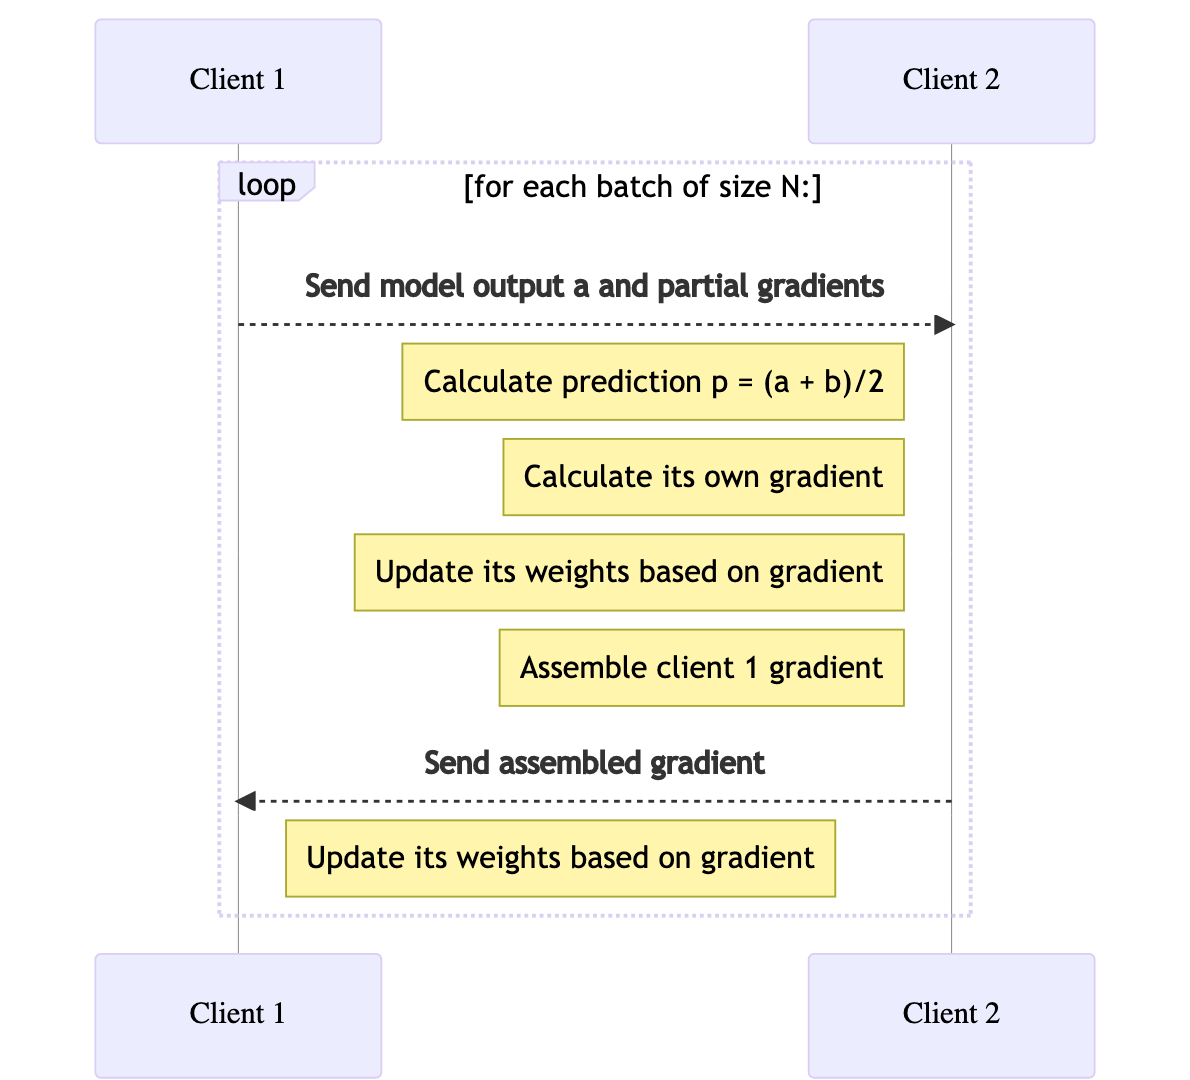
\includegraphics[width=0.6\textwidth]{./images/vfedcce_diagram2.png}
  \caption{Sequence diagram for \texttt{vFedCCE}}
  \label{vflseqdia}
\end{wrapfigure}

\paragraph{Correctness.} The correctness of \texttt{vFedCCE} depends on the gradients calculated or assembled locally on clients to update their respective weight vectors.

\begin{proof}
We study a batch of $N$ examples, where features $x_1^1,x_2^1,\ldots,x_N^1$ are stored on client 1, features $x_1^2,x_2^2,\ldots,x_N^2$ and labels $y_1,y_2,\ldots,y_N$ are stored on client 2 as one-hot arrays in $\mathbb{R}^m$, where $m$ is the number of classes to predict. On a single example $i$, the probability distribution output of client 1 on its feature set $x_i^1$ will be $a_i=w_1x_i^1$ and the probability distribution output of client 2 on its feature set $x_i^2$ will be $b_i=w_2x_i^2$. For the shared model, we aim to train the model such that the average output of the client outputs converges to the actual labels $y_i$. Therefore, the predicted probability distribution of the shared model will be $p_i=\frac{1}{2}(a_i+b_i)$. Note that all probability distributions, i.e. $a_i,b_i,y_{\text{pred},i}$ are vectors in $\mathbb{R}^m$.

Therefore, on this batch of $N$ examples, probability distribution outputs of client 1, client 2 and the shared model on them will be $N\times m$ matrices: $a=\begin{bmatrix}a_1&a_2&\ldots&a_N\end{bmatrix}^T$, $b=\begin{bmatrix}b_1&b_2&\ldots&b_N\end{bmatrix}^T$ and $p=\frac{1}{2}(a+b)$. On the other hand, the actual labels $y$ stored on client 2 is also a $N\times m$ matrix where $y=\begin{bmatrix}y_1&y_2&\ldots&y_N\end{bmatrix}^T$.

As previously mentioned, the shared model aims to converge $p$ towards $y$, and therefore, the optimization goal is to minimize the categorical cross entropy loss $p$ against $y$, which is
$$
  \mathcal{L}=-\frac{1}{N}\sum_{i=1}^N y_i \cdot \log p_i = -\frac{1}{N}\sum_{i=1}^N \sum_{j=1}^m y_{ij}\log p_{ij}=-\frac{1}{N}\sum_{i=1}^s \sum_{j=1}^m (y_i)_j\log \frac{(a_i)_j+(b_i)_j}{2}.
$$
When using a gradient-based optimizer to minimize $\mathcal{L}$, one must calculate the gradients $\frac{\mathcal{L}}{\partial w_1}$ and $\frac{\mathcal{L}}{\partial w_2}$. Note that only $a_{ij}$ instead of $b_{ij}$ or $y_{ij}$ is a function of $w_1$, then by calculus chain rule we have
\begin{equation}
  \label{client1}
  \frac{\partial\mathcal{L}}{\partial w_1}=-\frac{1}{N}\sum_{i=1}^N \sum_{j=1}^m y_{ij}\frac{2}{a_{ij}+b_{ij}}\frac{\partial a_{ij}}{\partial w_1}=-\frac{1}{N}\sum_{i=1}^N \sum_{j=1}^m\frac{y_{ij}}{p_{ij}}\frac{\partial a_{ij}}{\partial w_1}.
\end{equation}
Similarly, for client 2,
\begin{equation}
  \label{client2}
  \frac{\partial\mathcal{L}}{\partial w_2}=-\frac{1}{N}\sum_{i=1}^N \sum_{j=1}^m y_{ij}\frac{2}{a_{ij}+b_{ij}}\frac{\partial b_{ij}}{\partial w_2}=-\frac{1}{N}\sum_{i=1}^N \sum_{j=1}^m\frac{y_{ij}}{p_{ij}}\frac{\partial b_{ij}}{\partial w_2}.
\end{equation}

Note that for privacy reasons, the labels $y$ stored on client 2 are not allowed to leave client 2. Therefore, we cannot directly send $y$ to client 1 in order to complete the calculations from (\ref{client1}) entirely locally on client 1. However, it is possible to send example-wise partial gradients $\frac{\partial a_{ij}}{\partial w_1}$ to client 2 to assemble into the total gradient $\frac{\partial\mathcal{L}}{\partial w_1}$ with the assistance of $y$ and $p$, which is what the function \texttt{AssembleGradient()} does in Algorithm \ref{vflalgo}.

As for client 2, since the labels $y$ are originally stored there and client 1's model output $a$ is safe to send, it can complete the calculations from (\ref{client2}) entirely locally. If we denote the element wise division $y\oslash p$ as a constant matrix $c$, client 2's gradiant can be calculated as follows:

\begin{align*}
  \frac{\partial\mathcal{L}}{\partial w_2}&=-\frac{1}{N}\sum_{i=1}^N \sum_{j=1}^m\frac{y_{ij}}{p_{ij}}\frac{\partial b_{ij}}{\partial w_2}=-\frac{1}{N}\sum_{i=1}^N \sum_{j=1}^m c_{ij}\frac{\partial b_{ij}}{\partial w_2}\\
  &=\frac{\partial}{\partial w_2}\left(-\frac{1}{N}\sum_{i=1}^N\sum_{j=1}^m c_{ij} b_{ij}\right)
  =\frac{\partial}{\partial w_2}\left(-\frac{1}{N}\left\langle c,b\right\rangle_\mathrm{F}\right)
\end{align*} which is what the function \texttt{CalculateLossAndUpdate()} does in Algorithm \ref{vflalgo} to calculate the gradient for client 2.

Therefore, the gradients calculated locally on the clients in Algorithm \ref{vflalgo} equals the actual gradients of the loss funciton w.r.t. $w_1$ and $w_2$ respectively. With a specified gradient-based optimizer, the output of the shared model, i.e. the average model of clients' models, $p$ will eventually converge to $y$ to achieve desired learning outcomes.
\end{proof}

\paragraph{Theoretical performance.} Unlike \cite{hardy2017private} where a Taylor approximation of the loss function is used to apply vertical federated learning, \texttt{vFedCCE}, according to the previous proof, calculates the accurate gradients without approximation. Therefore, theoretically \texttt{vFedCCE} should produce the same training outcomes (i.e. accuracy et al) compared to a conventional machine learning algorithm with the same model over a combined dataset.

Except preserving privacy, one major advantage of vertical federated learning is to reduce communication cost by avoiding sending huge datasets from the clients to the server to combine and then apply conventional deep learning over it. Although compared with the VFL example from \cite{yang2019federated} which only sends local gradients $\frac{\partial L}{\partial w}$ (it is possible because they are dealing with a linear regression model and an $L^2$ regularized MSE loss function), much more amount of intermediate data is being sent in Algorithm \ref{vflalgo} when sending $\frac{\partial a_{ij}}{\partial w_1}$, we expect the communication cost will still be reduced when the dataset is too huge to efficiently send and combine on the server.

One potential issue with Algorithm \ref{vflalgo} is that, when assembling client 1's gradient from all the partial gradients $\frac{\partial a_{ij}}{\partial w_1}$, a lot of floating point arthmetic calculation is being carried out and mannually summed up, which may lead to a presicion problem compared with a conventional approach. This concern has been dismissed by the experimental results shown later in section \ref{vflexp}.

\paragraph{Privacy.} In order to analyse where Algorithm \ref{vflalgo} preserves privacy, we need to evaluate the data being sent across the clients, which, rdeferring to Figure \ref{vflseqdia}, is:
\begin{itemize}
  \item Client 1's model output $a=\begin{bmatrix} w_1x_1^1& w_1x_2^1& \ldots &w_1x_N^1 \end{bmatrix}^T$. This data is safe and necessary to send as the shared model needs to average the two outputs for predictions.
  \item Client 1's partial gradients $\frac{\partial a_{ij}}{\partial w_1}$. This is safe to send as client 2 cannot restore the $x$ values from partial derivatives $\frac{\partial a_{ij}}{\partial w_1}$. Also, gradients are being sent in other literature such as \cite{yang2019federated} and \cite{hardy2017private}.
  \item Client 1's total gradient, sent from client 2 to client 1. This is also safe and necessary to sent as this is the gradient client 1 needs to update its own weight vectors.
\end{itemize}

Although Algorithm \ref{vflalgo} only sent secure intermediate data instead of sensitive raw data, it is still important to discuss the feasibility of applying some encryption scheme on top of \texttt{vFedCCE}. In our case, since all the intermediate data (i.e. $a$ and $\frac{\partial a_{ij}}{w_1}$) is sent for linear operations, it seems to be possible to apply addictively homomorphic encryption on those data. However, more details on encryption will be discussed later.

\section{Implementation and experimental results}\label{vflexp}
\paragraph{Implementation details.} The proposed \texttt{vFedCCE} algorithm is implemented in Python with the TensorFlow Keras library on the vertically partitioned SGCP dataset from \cite{groemping2019south}. In the experiments, the local models on client 1 and client 2 are the same neural network model:
\begin{itemize}
  \setlength\itemsep{0em}
  \item one normalizer layer;
  \item two fully connected L2 regularized dense layers with dropout activated by \texttt{elu};
  \item one more dense layer of unit $2$ to convert output into logits;
  \item one \texttt{Softmax} layer to output probability distributions).
\end{itemize}
This neural network model is choosed because it leads to acceptable results with a conventional approach on the combined dataset, denoted by \texttt{combinedNN}, which is the baseline method to benchmark the performance of \texttt{vFedCCE}.

For hyperparameters, no deliberate tuning is being applied since the goal of experiments is to verify that the learning outcome of \texttt{combinedNN} and \texttt{vFedCCE} are similar, instead of to achieve perfect performance. Both methods are implemented with the same hyperparameters: the learning rate (of Adam optimizer) $\eta=0.001$, the number of epochs $E=50$ and the batch size $N=32$.

\paragraph{Experimental results.} Figure \ref{fig:vflexp} demonstrates the training loss and accuracy of \texttt{combinedNN} and \texttt{vFedCCE} under the implementation specified previously. It shows that the two methods are able to minimize loss and increase accuracy over epochs, with similar speed. Table \ref{vfltest} presents the learning outcome of the two methods, which, expected, shows both similar and acceptable accuracy, precision, recall, F-score and AUC values. This also dismisses the concern on floating-point precision raised in section \ref{vfedcce}.

\begin{figure}[h]
\centering
\begin{subfigure}{.5\textwidth}
  \centering
  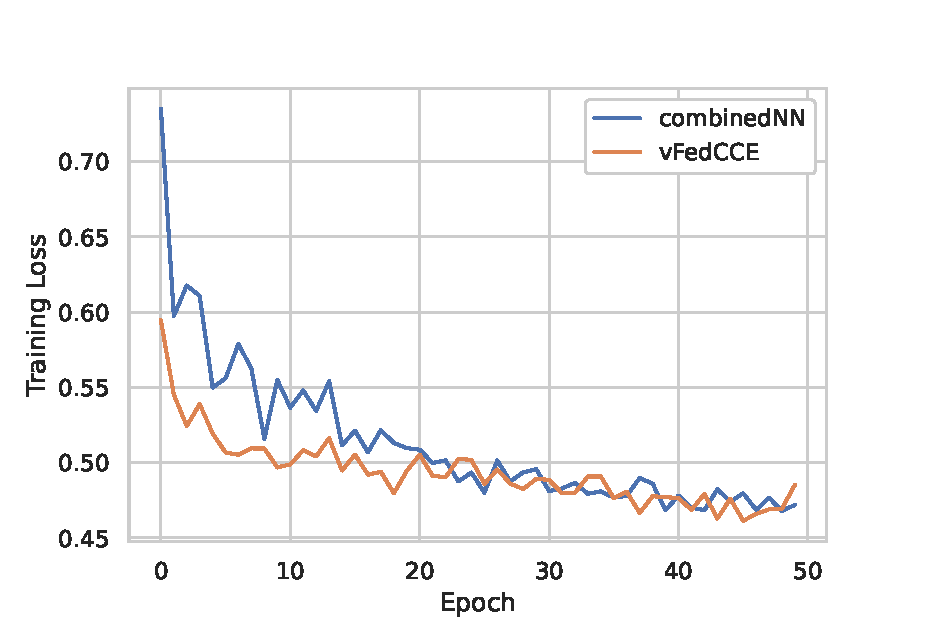
\includegraphics[width=\linewidth]{./images/vfl_train_loss.eps}
  \caption{Training loss over 50 epochs}
  \label{fig:vflloss}
\end{subfigure}%
\begin{subfigure}{.5\textwidth}
  \centering
  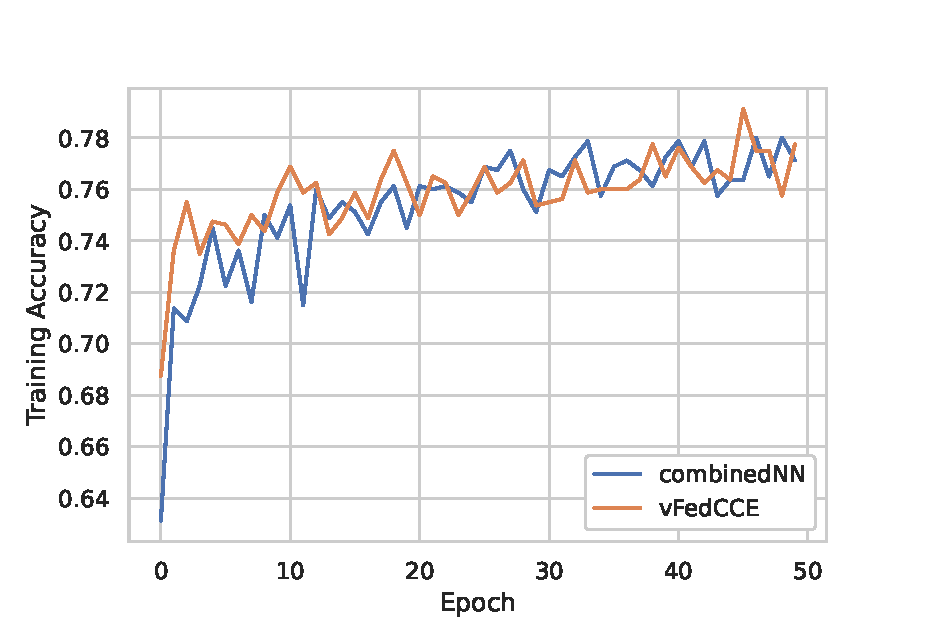
\includegraphics[width=\linewidth]{./images/vfl_train_acc.eps}
  \caption{Training accuracy over 50 epochs}
  \label{fig:vflacc}
\end{subfigure}
\caption{Training process of \texttt{vFedCCE} against \texttt{combinedNN}}
\label{fig:vflexp}
\end{figure}

\begin{table}[h]
\centering
  \resizebox{0.7\textwidth}{!}{%
  \begin{tabular}{|c|c|c|c|c|c|}
    \hline
                        & Accuracy & Precision & Recall & F-score & AUC    \\ \hline
    \texttt{combinedNN} & 0.74     & 0.7881    & 0.8561 & 0.9207  & 0.7720 \\ \hline
    \texttt{vFedCCE}    & 0.74     & 0.7669    & 0.8993 & 0.8278  & 0.7561 \\ \hline
  \end{tabular}%
  }
\caption{Learning outcome on testing data of \texttt{vFedCCE} against \texttt{combinedNN}}
\label{vfltest}
\end{table}

\bibliographystyle{abbrvnat}
\bibliography{references}
\end{document}